\documentclass[
  bibliography=totoc,     % Literatur im Inhaltsverzeichnis
  captions=tableheading,  % Tabellenüberschriften
  titlepage=firstiscover, % Titelseite ist Deckblatt
]{scrartcl}
%Bro wir wollen nur was drehen
\usepackage{rotating}
% Paket float verbessern
\usepackage{scrhack}

% Warnung, falls nochmal kompiliert werden muss
\usepackage[aux]{rerunfilecheck}

% unverzichtbare Mathe-Befehle
\usepackage{amsmath}
% viele Mathe-Symbole
\usepackage{amssymb}
% Erweiterungen für amsmath
\usepackage{mathtools}

% Fonteinstellungen
\usepackage{fontspec}
% Latin Modern Fonts werden automatisch geladen
% Alternativ zum Beispiel:
%\setromanfont{Libertinus Serif}
%\setsansfont{Libertinus Sans}
%\setmonofont{Libertinus Mono}

% Wenn man andere Schriftarten gesetzt hat,
% sollte man das Seiten-Layout neu berechnen lassen
\recalctypearea{}

% deutsche Spracheinstellungen
\usepackage[ngerman]{babel}


\usepackage[
  math-style=ISO,    % ┐
  bold-style=ISO,    % │
  sans-style=italic, % │ ISO-Standard folgen
  nabla=upright,     % │
  partial=upright,   % │
  mathrm=sym,        % ┘
  warnings-off={           % ┐
    mathtools-colon,       % │ unnötige Warnungen ausschalten
    mathtools-overbracket, % │
  },                       % ┘
]{unicode-math}

% traditionelle Fonts für Mathematik
\setmathfont{Latin Modern Math}
% Alternativ zum Beispiel:
%\setmathfont{Libertinus Math}

\setmathfont{XITS Math}[range={scr, bfscr}]
\setmathfont{XITS Math}[range={cal, bfcal}, StylisticSet=1]

% Zahlen und Einheiten
\usepackage[
  locale=DE,                   % deutsche Einstellungen
  separate-uncertainty=true,   % immer Unsicherheit mit \pm
  per-mode=symbol-or-fraction, % / in inline math, fraction in display math
]{siunitx}

% chemische Formeln
\usepackage[
  version=4,
  math-greek=default, % ┐ mit unicode-math zusammenarbeiten
  text-greek=default, % ┘
]{mhchem}

% richtige Anführungszeichen
\usepackage[autostyle]{csquotes}

% schöne Brüche im Text
\usepackage{xfrac}

% Standardplatzierung für Floats einstellen
\usepackage{float}
\floatplacement{figure}{htbp}
\floatplacement{table}{htbp}

% Floats innerhalb einer Section halten
\usepackage[
  section, % Floats innerhalb der Section halten
  below,   % unterhalb der Section aber auf der selben Seite ist ok
]{placeins}

% Seite drehen für breite Tabellen: landscape Umgebung
\usepackage{pdflscape}

% Captions schöner machen.
\usepackage[
  labelfont=bf,        % Tabelle x: Abbildung y: ist jetzt fett
  font=small,          % Schrift etwas kleiner als Dokument
  width=0.9\textwidth, % maximale Breite einer Caption schmaler
]{caption}
% subfigure, subtable, subref
\usepackage{subcaption}

% Grafiken können eingebunden werden
\usepackage{graphicx}

% schöne Tabellen
\usepackage{tabularray}
\UseTblrLibrary{booktabs, siunitx}

% Verbesserungen am Schriftbild
\usepackage{microtype}

% Literaturverzeichnis
\usepackage[
  backend=biber,
]{biblatex}
% Quellendatenbank
\addbibresource{lit.bib}
\addbibresource{programme.bib}

% Hyperlinks im Dokument
\usepackage[
  german,
  unicode,        % Unicode in PDF-Attributen erlauben
  pdfusetitle,    % Titel, Autoren und Datum als PDF-Attribute
  pdfcreator={},  % ┐ PDF-Attribute säubern
  pdfproducer={}, % ┘
]{hyperref}
% erweiterte Bookmarks im PDF
\usepackage{bookmark}

% Trennung von Wörtern mit Strichen
\usepackage[shortcuts]{extdash}

\author{%
  Benedikt Nelles\\%
  \href{mailto:authorA@udo.edu}{benedikt.nelles@tu-dortmund.de}%
  \and%
  Tom Bollig\\%
  \href{mailto:authorB@udo.edu}{tom.bollig@tu-dortmund.de}%
}
\publishers{TU Dortmund – Fakultät Physik}




\begin{document}





    \section{Theorie}
    	Eine Feder mit Federkonstante $\symbf{D}$ ist senkrecht zum Boden an einem Kraftmessgerät aufgehängt.
        Die Feder ist auf der anderen Seite mit einem Seil verbunden, dass über eine feste Rolle um 90° gedreht wird.
        Entlang dem Seil ist ein Lineal angebracht. Das Ende des Seils, wenn dieses locker hängt sollte sich dabei bei der Position 0$\unit{cm}$ befinden.

    \section{Durchführung}
        Das Seil wird um eine gewisse Entfernung entlang des Lineals ausgelenkt.
        Dann wird die Auslenkung vom Ruhezustand am Lineal abgelesen.
        Zusätzlich soll die Kraft am Kraftmessgerät abgelesen werden.
        Danach berechnet man die Federkonstante mit 
        \begin{equation}
            \symbf{D}=\frac{\symbf{F}}{\increment\symbf{x}}
        \end{equation}
    \section{Auswertung}
    \begin{table}
        \centering
        \caption{Messwerte}
        \sisetup{table-format=1.2}
        \begin{tblr}{
            colspec={S S S[table-format=1.0]},
            row{1}={guard, mode=math},
            }
            \toprule
            $\increment$x/\unit{\meter} & F/\unit{\newton} & D/\unit[per-mode=fraction]{\newton\per\meter} \\
            \midrule    
            0.05 & 0.15 & 3    \\
            0.1  & 0.29 & 2.9  \\
            0.15 & 0.44 & 2.93 \\
            0.2  & 0.59 & 2.95 \\
            0.25 & 0.74 & 2.96 \\
            0.3  & 0.89 & 2.97 \\
            0.35 & 1.04 & 2.97 \\
            0.4  & 1.19 & 2.98 \\
            0.45 & 1.34 & 2.98 \\
            0.5  & 1.49 & 2.98 \\
            \bottomrule
        \end{tblr}
    \end{table}
    Der Mittelwert der gemessenen Federkonstanten beträgt dabei 2,962$\unit[per-mode=fraction]{\newton\per\meter}$.\\
    Die Steigung der Regressionsgeraden beträgt 2,99$\unit[per-mode=fraction]{\newton\per\meter}$.
\begin{figure}
    \centering
    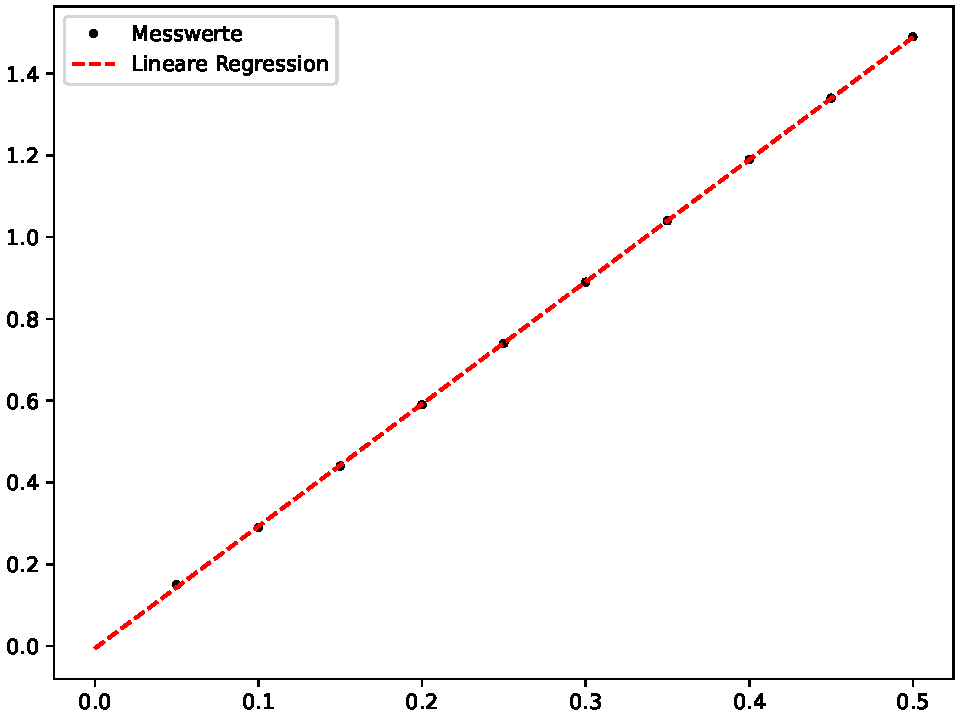
\includegraphics[width=\textwidth]{plot.pdf}
    \caption{Lineare Regression}
\end{figure}

\end{document}

